\lysh{34838}{4}
\begin{alist}
\item Για το τυχαίο σημείο $M$ της γραφικής παράστασης της συνάρτησης $f$ είναι:
\[ M(x, y) = (x, 2\sqrt{x}), x \ge 0 \]
Επομένως, η απόσταση $AM$, συναρτήσει του $x$, είναι:
\[ AM = d(x) = \sqrt{(x-3)^2 + (2\sqrt{x}-0)^2} \]
\[ = \sqrt{x^2 - 6x + 9 + 4x} \]
\[ = \sqrt{x^2 - 2x + 9}, x \ge 0 \]
\item Η ελάχιστη απόσταση θα παρουσιαστεί όταν το υπόριζο $x^2 - 2x + 9, x \ge 0$ γίνει ελάχιστο. Θεωρούμε τη συνάρτηση $g(x) = x^2 - 2x + 9, x \ge 0$.
Η συνάρτηση $g(x)$ είναι παραγωγίσιμη για $x \ge 0$ με
\[ g'(x) = (x^2 - 2x + 9)' = 2x - 2 \]
\[ g'(x) = 0 \Leftrightarrow 2x - 2 = 0 \Leftrightarrow x = 1 \]
\[ g'(x) > 0 \Leftrightarrow 2x - 2 > 0 \Leftrightarrow x > 1 \]
\[ g'(x) < 0 \Leftrightarrow 2x - 2 < 0 \Leftrightarrow x < 1 \]

Τα πρόσημα της παραγώγου της συνάρτησης $g(x)$ φαίνονται στον ακόλουθο πίνακα:
\begin{center}
\begin{tikzpicture}
\tikzset{arrow style/.style={maincolor,>->,>=latex'}}
\tikzset{t style/.style = {style = dashed}}
\tikzset{z style/.style = {fill=white,inner sep=.2mm}}
\tkzTabInit[color,lgt=2,espcl=2.4,colorC = maincolor,colorL = maincolor,colorV = maincolor]%
{$x$ / .8,$g'(x)$ /.8,$g(x)$/0.8}%
{$0$,$1$,$+\infty$}%
\tkzTabLine{,-,z,+,}
\tkzTabVar{,-/, ,+/}% This draws the decreasing and increasing arrows.
\end{tikzpicture}
\end{center}
Για τη συνάρτηση $g(x)$ ισχύουν $g'(1)=0$, $g'(x)<0$ στο $[0,1)$ και $g'(x)>0$ στο $(1,+\infty)$. Επομένως, η $g(x)$ παρουσιάζει ελάχιστο για $x=1$.
Άρα, η απόσταση $AM$ γίνεται ελάχιστη για το σημείο $M(1,2)$.
\item Η ελάχιστη απόσταση $AM$ ισούται με:
\[ d(1) = \sqrt{1^2 - 2 \cdot 1 + 9} = \sqrt{1 - 2 + 9} = \sqrt{8} \]
\end{alist}
\vspace{6mm}
\noindent\rule{\textwidth}{0.4pt}
\vspace{6mm}

